% Document class and packages
\documentclass[letterpaper, 12pt]{article}
\usepackage[utf8]{inputenc}
\usepackage[T1]{fontenc}
\usepackage{geometry}
\usepackage{titlesec}
\usepackage{enumitem}

\usepackage{amsmath, amssymb,lipsum,fancyhdr,graphicx,listings,xcolor,color,array}

% Page setup
\geometry{margin=1in}
\pagestyle{fancy}
\fancyhf{}
\rhead{\thepage}
\lhead{\textit{Audio \& Image Compression - Assignment 3 - Video}}  % Escape '&' with '\&'

% Section and list formatting
\titleformat{\section}[block]{\normalfont\Large\bfseries}{\thesection}{1em}{}[]
\setlist[itemize]{left=0pt, label=--, itemsep=4pt}

% Document information
\title{Audio \& Image Compression}
\author{Bashar Beshoti (207370248)
}
\date{\today}

\begin{document}

% First page: Course details and author information
\maketitle

\section*{Course Information}
\begin{itemize}
    \item \textbf{Course Title:} Audio \& Image Compression  % Escape '&' with '\&'
    \item \textbf{Course Code:} 203.3880
    \item \textbf{Assignment :} Final assignment - Video
    \item     \textbf{Due Date : } 04.04.2024

\end{itemize}


\definecolor{dkgreen}{rgb}{0,0.6,0}
\definecolor{gray}{rgb}{0.5,0.5,0.5}
\definecolor{mauve}{rgb}{0.58,0,0.82}

\lstset{frame=tb,
  language=Python,
  aboveskip=3mm,
  belowskip=3mm,
  showstringspaces=false,
  basicstyle={\small\ttfamily},
  numbers=none,
  numberstyle=\tiny\color{gray},
  keywordstyle=\color{blue},
  commentstyle=\color{dkgreen},
  stringstyle=\color{mauve},
  breaklines=true,
  tabsize=3,
  frame=single
}

\newpage

\section{Video Compression:}

\subsection{Traffic search} - A block of "pixels" must be built from a combination of digits based on your ID number. 8 must be taken
The last digits, in combinations of pairs of numbers in the following way:
Let's assume an identity number: \textbf{0 3 5 4 7 8 9 6 5} we will mark.\\

\textbf{The block will be structured as follows:}
i.e $a=35, b=47$ And so on.\\


\begin{table}[htbp]
    \centering
\caption{The Block}    \begin{tabular}{|c|c|c|c|c|} \hline 
         50&  47&  45&  48& 46\\ \hline 
         53&  a&  b&  40& 43\\ \hline 
         50&  46&  c&  39& 38\\ \hline 
         53&  50&  43&  d& 42\\ \hline 
         51&  45&  38&  45& 40\\ \hline
    \end{tabular}
    
    
\end{table}

A full motion search must be performed for the next block (from left to right from top to bottom):


\begin{table}[htbp]
    \centering
    \begin{tabular}{|c|c|} \hline 
         a& b\\ \hline 
         c& d\\ \hline
    \end{tabular}
\end{table}
When the search is within the boundaries of the 5x5 block and show:
\paragraph{1. What is the optimal position (movement vector) relative to the beginning of the axes (left corner (the upper one, a highlighted pixel with a value of 50)?}

\paragraph{Answer :} Let's find a,b,c,d based on my identity. since my identity number is 207370248. therefore $a = 07, b=37, c = 02 , d = 48$. The Block will look like: 
\begin{table}[htbp]
    \centering
    \begin{tabular}{|c|c|} \hline 
         07& 37\\ \hline 
         02& 48\\ \hline
    \end{tabular}
    \caption{Parameters a,b,c,d values respectively}
\end{table}
Therefore The block is:
\begin{table}[htbp]
    \centering
    \begin{tabular}{ccccc}
        50&  47&  45&  48& 46\\ 
         53&  07&  37&  40& 43\\
         50&  46&  02&  39& 38\\ 
         53&  50&  43&  48& 42\\ 
         51&  45&  38&  45& 40\\
    \end{tabular}
    \caption{The Block after putting a,b,c,d values}
\end{table}

\newpage

\paragraph{2. What is the SAD in this case?}
\paragraph{Answer :}
For instance, 

\begin{align*}
    SAD(0,0) = \sum_{i=0}^{N-1}\sum_{j=0}^{N-1}(|curr\_block(i,j) - ref\_region(i,j)|) \\
    = |50 - 7| +|47-37| + |53-02|+|7-48| = 43 + 10 + 51 + 41 = 145
\end{align*}

The Minimum SAD: 

\[SAD(1,2) = \sum_{i=0}^{N-1}\sum_{j=0}^{N-1}(|curr\_block(i,j) - ref\_region(i,j)|)\]
\[= |37 - 7| +|40-37| + |2-2|+|39-48| = 30 + 3 + 0 + 9 = 42\]

So, the movement vector is $(1-0.2-0) = (1,2)$ . \\
\newpage
\textbf{The Code i used to calculate SAD value over each block 2x2 in Matrix.}
\begin{lstlisting}
def calculate_sad(matrix, ref_region):
    sad_values = []
    min_sad = float('inf')
    min_index = None
    min_matrix = None

    for i in range(len(matrix) - 1):
        row_sads = []
        for j in range(len(matrix[0]) - 1):
            sad = 0
            for x in range(2):
                for y in range(2):
                    sad += abs(matrix[i + x][j + y] - ref_region[x][y])

            row_sads.append(sad)
            if sad < min_sad:
                min_sad = sad
                min_index = (i, j)
                min_matrix = [row[j:j+2] for row in matrix[i:i+2]]

        sad_values.append(row_sads)

    return sad_values, min_sad, min_index, min_matrix

# Given matrix
matrix = [
    [50, 47, 45, 48, 46],
    [53, 7, 37, 40, 43],
    [50, 46, 2, 39, 38],
    [53, 50, 43, 48, 42],
    [51, 45, 38, 45, 40]
]

# Reference region
ref_region = [
    [7, 37],
    [2, 48]
]

# Calculate SAD for each 2x2 block and find the minimum SAD value along with its index and the corresponding 2x2 matrix
sad_values, min_sad, min_index, min_matrix = calculate_sad(matrix, ref_region)

# Print SAD values in a table format
print("SAD Values Table:")
for i in range(len(sad_values)):
    for j in range(len(sad_values[0])):
        print(f"{sad_values[i][j]:<5}", end=" ")
    print()

# Print the minimum SAD value, its corresponding index, and the 2x2 matrix with the minimum SAD
print("\nMinimum SAD:", min_sad)
print("Index with minimum SAD:", min_index)
print("2x2 Matrix with minimum SAD:")
for row in min_matrix:
    print(row)


\end{lstlisting}
\textbf{OUTPUT} :
\begin{lstlisting}
SAD Values Table:
145   64    92    93    
126   90    42    86    
105   127   48    85    
111   102   86    97    

Minimum SAD: 42
Index with minimum SAD: (1, 2)
2x2 Matrix with minimum SAD:
[37, 40]
[2, 39]
=== Code Execution Successful ===

\end{lstlisting}
\paragraph{3. How many search steps are required - It is recommended to show a SAD table for every move!}
\paragraph{Answer :} The number of search steps would be equal to the number of possible positions for the 2x2 block within the 5x5 block. Since the 2x2 block can be positioned in a 4x4 region within the 5x5 block, there would be 16 possible positions, and therefore, 16 search steps.

\begin{table}[htbp]
    \centering
        \caption{SAD Values Table:}

    \begin{tabular}{|c|c|c|c|} \hline 
         145&  64&  92& 93\\ \hline 
         126&  90&  42& 86\\ \hline 
         105&  127&  48& 85\\ \hline 
         111&  102&  86& 97\\ \hline
    \end{tabular}
\end{table}


\paragraph{4. Is it guaranteed that in a different type of search - for example Conjugate, hierarchical, random, etc. we will reach it outcome ? It is necessary to reason well with the help of a simple demonstration?}
\paragraph{Answer :} \textbf{Guarantee of Optimal Outcome with Different Searches:} \\
\begin{enumerate}
    \item Full Search: Guaranteed to find the optimal position within the search area (boundaries of the block in this case). It checks all possible movements, making it computationally expensive.
    \item Conjugate Search: This starts with a full search in a small diamond pattern around the initial position. If a minimum is found outside the diamond, it performs another search around that new minimum. While faster than full search, it might miss the global minimum in some cases.
    \item Hierarchical Search: This breaks down the search area into a hierarchy of grids with decreasing resolution. It first searches at a coarse level and then refines around promising regions at higher resolutions. This can be faster than full search but might miss the optimal position depending on the coarseness of the hierarchy.
    \item Random Search: This randomly samples positions within the search area. It's very fast but highly unlikely to find the optimal position consistently.
\end{enumerate}

\textbf{Demonstration}\textbf{:} \\
\begin{enumerate}
    \item Conjugate search might also find it quickly if the diamond pattern covers the distinct pattern.
    \item Hierarchical search might miss it if the coarsest level doesn't capture the distinct pattern initially.
    \item Random search would be highly unlikely to find it consistently.
\end{enumerate}


\subsection{In the 264H standard: there are some significant improvements:}
\begin{itemize}
    \item In traffic search: optimal division into blocks
    \item Prediction in intra-pictures
    \item Using iDCT instead of normal DCT
\end{itemize}

Regarding each of them, it is necessary to explain what its effect is on:
\begin{itemize}
    \item Final bit rate
    \item The quality of the restored image
    \item The complexity of the calculation
\end{itemize}
\paragraph{Answer :\\} 

\subparagraph{A. OPTIMAL DIVISION INTO BLOCKS:}

\begin{enumerate}
    \item \textbf{Final Bit Rate:} Through optimal division into blocks can lead to better compression efficiency within more accurate motion estimation results in less amount of data need to be encoded therefore, reducing the final bit rate. 
    \item \textbf{Quality of the Restored Image:} Upon optimal division, The optimal division into blocks allows smaller blocks to capture more local variations in pixel intensity, leading to a higher quality restored image when decoded. This results in reduced artifacts, prediction error and better visuals.
    \item \textbf{Complexity of Calculation:} From optimal division into blocks, it may also increase computational complexity during encoding as more potential block divisions need to be considered. The encoder needs to analyze each frame to determine the best partitioning strategy, which can require additional processing resources.
\end{enumerate}

\subparagraph{B. PREDICTION IN INTRA PICTURES:}

\begin{enumerate}
    \item \textbf{Final Bit Rate:} Intra-picture prediction exploits spatial correlations within a frame, resulting in more efficient compression. By predicting pixel values based on neighboring pixels within the same frame, the encoder can reduce the amount of residual information needed to represent the frame accurately. This leads to a lower final bit rate compared to encoding each frame independently.
    \item \textbf{Quality of the Restored Image:} Intra-picture prediction helps preserve fine details and textures within a frame by utilizing spatial redundancy effectively. therefore, the decoder can reconstruct the frame with fewer errors and reduced amount of artifacts.
    \item \textbf{Complexity of Calculation:} Prediction in Intra-pictures adds computational complexity to the encoding process since it requires analyzing neighboring pixels and selecting the best prediction mode for each block. 
\end{enumerate}

\subparagraph{C. USING IDCT INSTEAD OF NORMAL DCT:}

\begin{enumerate}
    \item \textbf{Final Bit Rate:} The use of iDCT does not directly affect the final bit rate, as it is a part of the decoding process. 
    \item \textbf{Quality of the Restored Image:} The use of iDCT can affect the quality of the restored image, as inaccuracies in algebra operations in the transform or inverse can lead to decoding errors and more distortion or artifacts.
    \item \textbf{Complexity of Calculation:} The use of iDCT decreases the complexity of the calculation, implemented using only additions and 
bit-shifting operations without multiplications.
\end{enumerate}


\subsection{On the next page are given the different infra prediction modes in the 264H standard.Use the block you created in section A:}
\begin{table}[htbp]
    \centering
    \caption{Original Block}
    \begin{tabular}{|c|c|c|c|c|c|c|c|c|} \hline 
         50&  47&  45&  48&  46&  46&  48&  45& 47\\ \hline 
         53&  7&  37&  42&  43&  &  &  & \\ \hline 
         50&  46&  2&  39&  38&  &  &  & \\ \hline 
         53&  50&  3&  48&  42&  &  &  & \\ \hline 
         51&  45&  38&  45&  40&  &  &  & \\ \hline
    \end{tabular}
\end{table}

Where the top row and the left column in it will be considered as the row and column of the blocks above and to the left Infra prediction must be performed according to the standard when the prediction mode will be determined according to the check digit in the number your identity For example, in the identity number above, the ninth digit which is the check digit is 5 and therefore Prediction method 5 (right-vertical).\\

\textbf{Note : there is no way of predicting, 9 whoever this is his check digit will use one digit to the left of the identity number}\\

It must be clearly and explicitly shown which method of prediction was chosen and the calculation formulas you used!
After performing the prediction for a block, find the prediction error block and calculate MSE for it.

\newpage
\paragraph{Answer :} My ID number is 207370248. Then, Prediction Mode 8 (Horizontal-Up).
\begin{figure}[htbp]
    \centering
            \caption{Prediction Mode 8}

    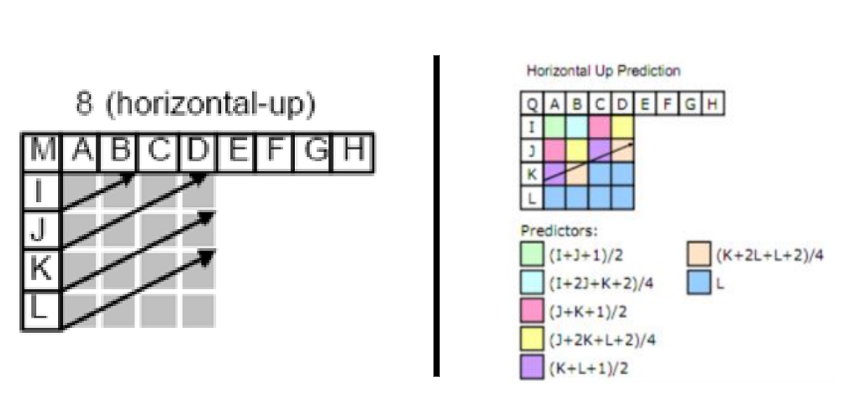
\includegraphics[width=0.75\linewidth]{FINAL_ASSIGNMENT/Prediction Mode.png}
    
\end{figure}

Let's calculate each predictor value: \\
1.
\[(I+J+1)/2 = (53+50+1)/2 = 52\]

2.
\[(I+2J+K+2)/4 = (52+2\cdot 50 + 53 + 2)/4 = 51.75\]
3.
\[(J+K+1)/2 = (50 + 53 + 1)/2 = 52\]
4.
\[(J+2K+L+2)/4 = (50 + 2 \cdot 53 + 51 + 2)/4 = 52.25\]
5. 
\[(K+L+1)/2 = (53 + 51 + 1)/2 = 52\]
6. 
\[(K+2L+L+2)/4 = (53 + 2 \cdot 51 + 51 + 2)/4 = 52\]

7.
\[(L) = 51\]

Evaluating a pixel value upon prediction as it written above. we notice 2 real numbers $(52.25,51.75)$. Pixel values allows only integers, therefore we use nearest neighbor of the value through rounding it to the closet integer which are $52$ for both of them.

\begin{table}[htbp]
    \centering
    \caption{Prediction Block}
    \begin{tabular}{|c|c|c|c|c|c|c|c|c|} \hline 
         50&  47&  45&  48&  46&  46&  48&  45& 47\\ \hline 
         53&  52&  52&  52&  52&  &  &  & \\ \hline 
         50&  52&  52&  52&  52&  &  &  & \\ \hline 
         53&  52&  52&  51&  51&  &  &  & \\ \hline 
         51&  51&  51&  51&  51&  &  &  & \\ \hline
    \end{tabular}
\end{table}
\textbf{Calculation:\\}
\begin{figure}
    \centering
    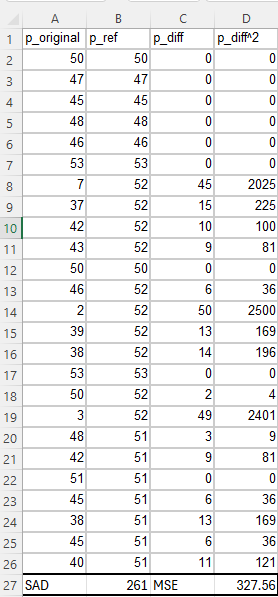
\includegraphics[width=0.5\linewidth]{FINAL_ASSIGNMENT/V_S_3.png}
    
    
\end{figure}

\begin{align*}
    MSE = \frac{1}{n^2}\sum(P_{source}-P(Quantized))^2 = 327.56
\end{align*}


\subparagraph{\textbf{Do you think the prediction was successful?}}
Based on the relatively high MSE and SAD values, it seems that the prediction was not very successful. The large errors between the original block and the reference block indicate that the prediction did not capture the underlying patterns or structure well.


\subparagraph{\textbf{Do you see another way of predicting that could be more successful? name reasons}}
One alternative prediction method that could potentially be more successful is using spatial intra prediction modes, such as vertical, horizontal, or diagonal prediction. These modes utilize neighboring pixels within the same frame to predict the value of a pixel. Since these methods directly use nearby pixel values rather than relying on a reference block from a different frame, they may provide more accurate predictions, especially for frames with less motion. 




\end{document}
